\section{Scala}
\subsection{Introduction}
Scala belongs to the group of programming languages that can be compiled into Java byte code and run on a Java virtual machine (JVM). The major part, which makes it different from well-known Java, is the combination of applying a functional approach with an object-oriented paradigm. 

\subsection{Functional error handling}
Scala avoids the usual \texttt{try catch} error handling, which is used in Java. The only occasion where it might be used is when we are calling some Java API or unsafe library. Instead, Scala is using monads, for example, \texttt{Option[T]}, \texttt{Try[T]}, and \texttt{Either[A, B]}. Monad is in simple terms container around a certain type, for which there is a \texttt{flatMap} function, which allows us to compose their individual instances.
\begin{itemize}
    \item \textbf{Option[T]} \\
        \texttt{Option} is definition of nullable type. It contains either \texttt{None} or \texttt{Some(T)} object. For example, we're trying to find a certain number in the \texttt{List[Int]}. We define a function that will traverse the list, and if the value is present, it returns the number, wrapped like this \texttt{Some(Int)}. If the value is not found, it returns \texttt{None}.
    \item \textbf{Either[A, B]} \\
        \texttt{Either} is similar to \texttt{Option}, but instead of returning simple \texttt{None}, which does not tell us what went wrong, it returns \texttt{Left(A)} or \texttt{Right(B)} object. \texttt{Right} is just like \texttt{Some}, it's returned when everything went right and we got the expected result. On the other hand, we return \texttt{Left} whenever something did not go as planned. It can contain info about the problem.
    \item \textbf{Try[T]} \\
        \texttt{Try} is more specific \texttt{Either}. It is the same as \texttt{Either[Throwable, B]}. The difference is that instead of \texttt{Right} there is \texttt{Success} and instead of \texttt{Left} there is \texttt{Failure}. However, \texttt{Failure} can be only exception. It is mostly used as replacement in situations, where we would use \texttt{try catch} block.
\end{itemize}

\subsection{Static vs. dynamic typing}
Besides the functional fundamentals, Scala belongs to the family of statically typed languages. This family also includes languages like C, C++, Java, or Haskell. Therefore, every single statement in Scala has a type.\cite{Static vs dynamic} Statically typed languages validate the type during compile time and once it is compiled, it can be run multiple times.

On the other hand, dynamic typing does all type checking during runtime, and every time we want to run the program, it has to be compiled again. Examples of languages, which use dynamic typing, are Python, Ruby, and PHP.

\subsection{Strong vs. weak typing}
Strongly typed languages enforce strict restrictions on intermixing values with different data types. Thanks to that, the behavior is more predictable than it would be for weakly typed language. The majority of strongly typed languages require explicit declaration of type for each variable. However, for Scala, that's not entirely true. It is strongly typed language, but it uses a system known as type inference - automatic type detection. That allows faster coding, thanks to the fact that we don’t have to worry about specifying the type for every statement. 

\begin{figure}[h]
  \makebox[\textwidth]{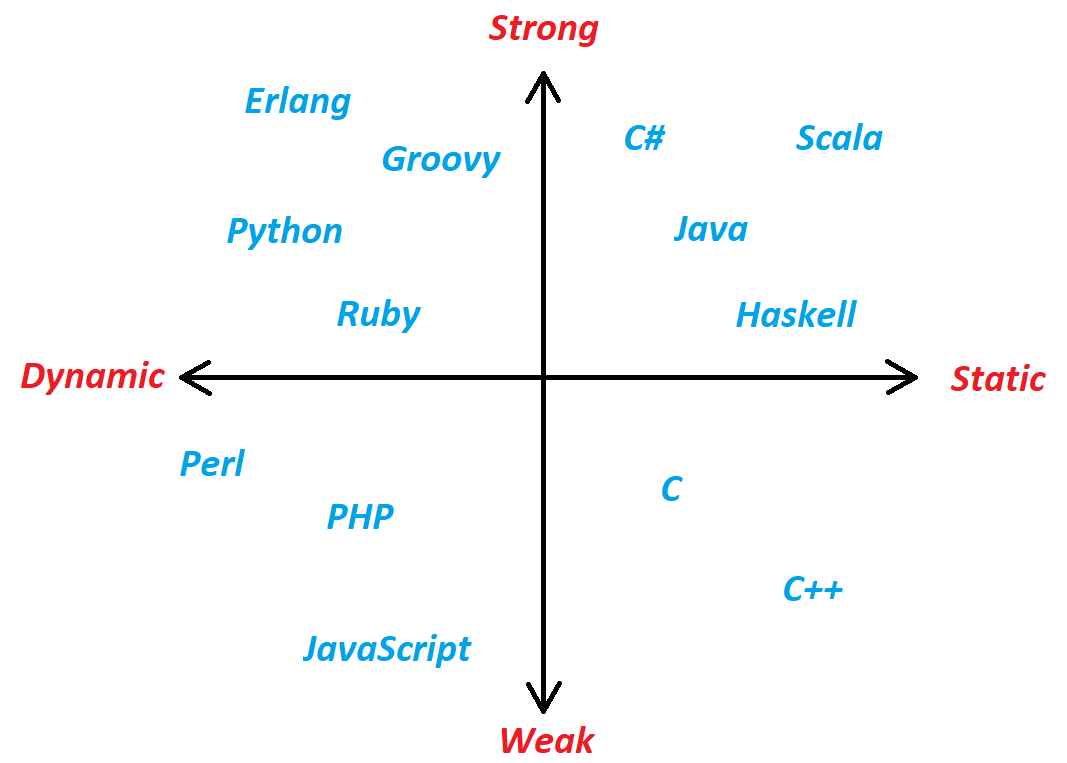
\includegraphics[width=\textwidth]{ownLanguage.png}}
  \caption {Languages divided into groups.}
\end{figure}

